\documentclass[11pt]{article}

\usepackage{amsmath}
\usepackage{amssymb}
\usepackage{booktabs}
\usepackage{graphicx}
\graphicspath{{figures/}}
\usepackage[margin=1in]{geometry}
\usepackage{hyperref}
\usepackage{parskip}
\usepackage{subcaption}
\hypersetup{colorlinks=true, linkcolor=blue, citecolor=blue, urlcolor=blue}

\newcommand{\Prob}{\mathbb{P}}
\newcommand{\E}{\mathbb{E}}
\newcommand{\sgn}{\operatorname{sign}}
\newcommand{\KL}{D_{\mathrm{KL}}}

\begin{document}
\author{Brecht Kerckhove\thanks{Personal project. The views expressed in this paper are solely those of the author and do not represent the views of any employer or affiliated organisation.}}
\date{\today}
\title{A Market-Implied Expected-Points Model for\\ World Cup Exact-Score Prediction}
\maketitle

\begin{abstract}
We describe the mathematical model behind an exact-score prediction engine for a
World Cup prediction pool with a custom, tiered scoring rule. The central idea is
that exact-score prediction is not a most-likely-outcome problem but an
\emph{expected-points optimisation} problem: the prediction that maximises expected
pool points under the scoring rule generally differs from the modal scoreline.
Bookmaker odds are treated as market-implied information. Decimal odds are converted
into devigged probabilities, which calibrate a scoreline probability matrix over
football scores; auxiliary markets (total goals, both-teams-to-score, Asian handicap,
correct score) supply additional structure. Predictions are then chosen by maximising
expected points over the matrix. We report an extended validation over $144$
group-stage matches from the 2014, 2018, and 2022 World Cups using a common 1X2
input set, alongside a richer 2018/2022 diagnostic layer with explicit
auxiliary-market inputs. The final policy is deliberately conservative: the
expected-points-optimal prediction is the live default, while modal,
market-consistent, Asian-handicap, and correct-score variants are retained as
challenger diagnostics or gated alternatives rather than automatic overrides. This
is a decision model for a scoring-rule contest, not a betting strategy, and we make
no claim of market-beating returns.
\end{abstract}

\textbf{Keywords:} prediction pool, expected-points optimisation, exact-score prediction, Poisson score model, market-implied probabilities, bookmaker odds

\clearpage
%########################################################################################

\section{Introduction}

Prediction pools are a familiar part of major sports tournaments such as the FIFA World Cup. Participants submit predictions for a sequence of matches and receive points according to how close those predictions are to the realised outcomes. One common format is an exact-score pool, where the participant predicts the final score of each match. At first sight, this looks like a simple forecasting problem: find the most likely scoreline and submit it. That instinct is not always correct.

The reason is that an exact-score pool is governed by a payoff table. A score such as 1-0, 1-1, or 2-1 may be the single most likely outcome, but the prediction that maximises expected pool points depends on the full scoring rule. If the pool awards partial credit for the correct winner or the correct goal difference, then a prediction should be judged by the points it earns across all possible outcomes, not only by the probability of hitting the exact score.

This turns exact-score prediction into a decision problem. The model still needs a probability distribution over scorelines, but the final prediction is chosen by passing that distribution through the pool's payoff function. In that sense, the problem is closer to pricing a payoff than to producing a simple point forecast: the same probability model can lead to different optimal predictions under different scoring rules.

The next question is where the scoreline probabilities should come from. In this project, the information backbone is the betting market. Bookmaker odds are useful because they compress a large amount of information into one price: historical team strength, current form, injuries, team news, trader judgement, market competition, risk management and betting flow. 

This approach is consistent with the broader quantitative evolution of football, where data-driven methods have become increasingly embedded in both sporting decisions and betting markets. In football specifically, odds-setters have been studied as forecasters, with bookmaker prices interpreted as implicit probabilistic forecasts of match outcomes \cite{forrest2005}. The same quantitative shift is visible in the betting industry itself: specialist firms such as Starlizard analyse large-scale sporting and betting-market data to produce betting probabilities and compare their real-time prediction systems with market prices.\footnote{Starlizard Integrity Services describes Starlizard's core business as analysing large amounts of sporting and betting-market data, converting this information into betting probabilities, and comparing betting markets with real-time prediction modelling systems.}

Therefore, after \emph{devigging}, meaning the removal of the bookmaker margin, bookmaker odds can be interpreted as market-implied probabilities. This does not mean that these probabilities are identical to the true physical probabilities of the match. Like prices in financial markets, they aggregate information but may also contain risk premia, liquidity effects, customer-demand effects and behavioural biases.

This finance analogy also guides the modelling pipeline: infer probabilities from market prices, calibrate a model to those prices, and optimise a decision under an explicit payoff function. In the present setting, the calibrated object is a scoreline distribution. The football literature has long used Poisson-type count models for this purpose \cite{maher1982,dixoncoles1997}, and has also studied both the information content and possible inefficiencies of betting markets \cite{dixoncoles1997}.

The aim of this model is to build a disciplined prediction-pool decision model and does not claim a betting edge. In a market where odds are already highly informative, the realistic source of improvement is not necessarily superior probability estimation, but the consistent translation of market-implied probabilities into decisions under the scoring rule.


\paragraph{Contributions.} This note makes four contributions. (i) It gives a formal
expected-points formulation of exact-score prediction under a tiered scoring rule, and a
closed-form decomposition that explains why the optimal prediction departs from the modal
scoreline. (ii) It describes a market-implied scoreline probability matrix calibrated to
liquid bookmaker markets rather than to historical goal counts. (iii) It catalogues a set of
challenger views --- modal, market-consistent / entropy-projected, Asian-handicap, and
correct-score --- as explainable diagnostics rather than automatic overrides. (iv) It
reports historical validation on the 2014, 2018, and 2022 World Cup group stages and
distils it into a conservative governance policy for live use.

\paragraph{Conceptual pipeline.} The model is a short chain in which each stage has a single
responsibility:
\[
\text{bookmaker odds}
\rightarrow
\text{devigged probabilities}
\rightarrow
\text{scoreline matrix}
\rightarrow
\text{market calibration}
\]
\[
\rightarrow
\text{expected-points optimisation}
\rightarrow
\text{challenger diagnostics}
\rightarrow
\text{validation / decision governance}.
\]
Sections~\ref{sec:calibration} onward follow this order: the first stages estimate the
scoreline matrix $\pi$, the optimisation stage turns $\pi$ into a prediction, and the final
stages stress-test and govern that prediction.

\section{The decision problem}

Let the realised scoreline of a match be a pair of non-negative integers
\[
(X,Y)\in\mathbb{N}_0^2,
\]
where $X$ and $Y$ are the goals of team A and team B. A prediction is a chosen scoreline
\[
p=(a,b)\in\mathbb{N}_0^2 .
\]
The model summarises beliefs about the match in a \emph{scoreline probability matrix}
\[
\pi_{xy}=\Prob(X=x,\,Y=y),\qquad \pi_{xy}\ge 0,\qquad \sum_{x,y}\pi_{xy}=1 .
\]
Although the Poisson distribution has infinite support, the model evaluates the scoreline matrix on a finite grid \(0 \leq x,y \leq G\). Let
\[
S_G
=
\sum_{i=0}^{G}\sum_{j=0}^{G} \pi_{ij}
\]
denote the probability mass retained on this grid. The working probability matrix is then the renormalised matrix
\[
\tilde{\pi}_{xy}
=
\frac{\pi_{xy}}{S_G},
\qquad
0 \leq x,y \leq G.
\]
The omitted tail mass is \(1-S_G\). For ordinary football matches this tail mass is typically negligible, while for extreme-favourite or high-total matches it is monitored through tail-mass and larger-grid diagnostics. In the implementation used for the historical validation below, the default grid is \(G=8\), so the working matrix covers scorelines from \(0\)-\(0\) up to \(8\)-\(8\).
For notational simplicity, the remainder of the paper writes this working renormalised finite-grid matrix again as \(\pi\), unless the distinction from the infinite-support Poisson distribution is material.

Given a scoring function
$g(p;X,Y)$ that returns the pool points earned when prediction $p$ meets outcome
$(X,Y)$, the optimal prediction maximises expected points:
\begin{equation}
p^{*}
=\arg\max_{(a,b)}\;\E\!\left[g\big((a,b);X,Y\big)\right]
=\arg\max_{(a,b)}\;\sum_{x,y}\pi_{xy}\,g\big((a,b);x,y\big).
\label{eq:objective}
\end{equation}
Equation~\eqref{eq:objective} is the core of the project. Everything upstream exists to
estimate $\pi$; everything downstream is a way to compute, explain, or stress-test
$p^{*}$.

In implementation, both the expectation and the candidate predictions are evaluated on a finite practical score grid; the omitted tail mass is tracked separately as a diagnostic.

%########################################################################################

\section{Scoring rule and expected-points decomposition}

The scoring rule used in this project follows the \emph{Sporza WK-pronostiek} format,\footnote{The \emph{Sporza WK-pronostiek} is a public World Cup prediction game run by Sporza in which participants predict match scorelines and can compete in private leagues with friends, family or colleagues.} but the model can be applied to any exact-score pool with a known payoff table. The scoring format is as follows:
\begin{equation}
g(p;X,Y)=
\begin{cases}
10, & (a,b)=(X,Y)\quad\text{(exact score)},\\[2pt]
7,  & a-b=X-Y\ \text{and}\ (a,b)\neq(X,Y)\quad\text{(goal difference)},\\[2pt]
5,  & \sgn(a-b)=\sgn(X-Y)\ \text{and}\ a-b\neq X-Y\quad\text{(result)},\\[2pt]
1,  & \text{otherwise (participation).}
\end{cases}
\label{eq:scoring}
\end{equation}
The tiers are nested: an exact score implies a correct goal difference, which implies a
correct result. Writing the realised margin $M=X-Y$ and the predicted margin $m=a-b$, we
can rewrite the expected score of equation~\eqref{eq:objective} as a sum of tier
increments. For a \emph{decisive} prediction ($m\neq 0$),
\begin{equation}
\E[g]
=1
+4\,\Prob\!\big(\sgn(M)=\sgn(m)\big)
+2\,\Prob(M=m)
+3\,\pi_{ab},
\label{eq:decisive}
\end{equation}
and for a \emph{draw} prediction ($m=0$), where ``correct result'' and ``correct goal
difference'' coincide,
\begin{equation}
\E[g]
=1
+6\,\Prob(M=0)
+3\,\pi_{aa}.
\label{eq:draw}
\end{equation}
The coefficients $\{1,4,2,3\}$ and $\{1,6,3\}$ are the differences between adjacent point
tiers; they follow directly from~\eqref{eq:scoring}.

These decompositions explain a subtle and practically important point. The exact-cell
term $3\pi_{ab}$ rewards the modal scoreline, but it is only one of several terms. For a
decisive prediction the optimiser also collects a large result-tier mass
($4\,\Prob(\sgn M=\sgn m)$) and a margin-tier mass ($2\,\Prob(M=m)$). In a balanced match
the most likely \emph{single} scoreline is often a draw such as $1\text{-}1$, yet a narrow
decisive prediction such as $1\text{-}0$ can have higher expected points because it earns
result credit across an entire half of the outcome space. Consequently the
expected-points-optimal pick is frequently a low-scoring decisive scoreline, and the modal
prediction is not automatically optimal. Whether a draw-leaning or modal prediction
outperforms in realised points depends on how a particular tournament happens to fall, a
theme we return to in Section~\ref{sec:validation}.

\section{Market-implied probabilities}

Each quoted decimal odd $O_i$ on a mutually exclusive, exhaustive set of outcomes implies
a raw inverse-odds probability
\[
q_i=\frac{1}{O_i}.
\]
Because bookmaker prices embed a margin, the raw probabilities sum to an overround
$R=\sum_i q_i>1$ and must be \emph{devigged}. The default and most conservative method is
normalised inverse odds,
\begin{equation}
p_i=\frac{q_i}{\sum_j q_j},
\label{eq:devig}
\end{equation}
which simply rescales by the overround. Alternative methods are available as diagnostics:
the \emph{power} method solves $\sum_i q_i^{\alpha}=1$ for an exponent $\alpha$ and sets
$p_i\propto q_i^{\alpha}$; the \emph{additive} method subtracts $(R-1)/n$ from each $q_i$;
and the \emph{Shin} method models the overround as arising partly from informed traders
and solves for a market-level parameter \cite{shin1993}. These methods differ mainly in
how they redistribute margin between favourites and longshots.

We prefer robust, conservative devigging for two reasons. First, the markets differ
structurally: two- and three-way markets (result, BTTS, totals) behave very differently
from many-outcome correct-score markets, which are sparse and carry large overrounds, so a
method tuned for one can distort another. Second, diagnostic backtests did not support
promoting the more aggressive power method for serious live use. Per-market devigging
therefore defaults to normalised inverse odds, with
a safe fallback when a diagnostic method fails to produce a valid probability vector for a
given market.

\paragraph{Market-implied versus physical probabilities.} The output of
equation~\eqref{eq:devig} is a \emph{market-implied} probability, not a claim about physical
truth. Beyond the explicit margin, quoted prices can embed a favourite--longshot bias, public
or sentiment-driven flow on popular nations, and possible risk premia, so the devigged
distribution may differ systematically from the true outcome distribution. This is the sports
analogue of the distinction between the risk-neutral and physical measures in derivatives
pricing: market prices are an information-efficient, internally consistent summary that is
expensive to beat, but they are not the data-generating process. We therefore use market
probabilities as a strong \emph{prior} rather than as ground truth --- the model calibrates to
them, but the validation in Section~\ref{sec:validation} tests the resulting distribution on
realised outcomes rather than assuming the market was correct.

%#############################################################################################
\section{Baseline scoreline model}

The baseline distribution treats goals as independent Poisson counts \cite{maher1982},
\[
X\sim\operatorname{Poisson}(\lambda_X),\qquad
Y\sim\operatorname{Poisson}(\lambda_Y),
\]
so that
\begin{equation}
\pi_{xy}
=\frac{e^{-\lambda_X}\lambda_X^{x}}{x!}\,
 \frac{e^{-\lambda_Y}\lambda_Y^{y}}{y!}.
\label{eq:poisson}
\end{equation}
The two intensities $(\lambda_X,\lambda_Y)$ are not estimated from raw historical goals but
\emph{calibrated to market-implied information} (Section~\ref{sec:calibration}), so the
matrix inherits the market's view of the match. The grid is truncated at a maximum goal
count $G$ and renormalised; the omitted tail mass is reported as a diagnostic, and a
larger-grid recomputation is available for extreme favourites. Independent Poisson is a
deliberately transparent baseline: it has only two parameters, it reproduces the standard
result, totals, and BTTS identities in closed form, and it is straightforward to audit. Its
known limitation --- mild dependence between the two scores, especially in low-scoring games
--- motivates the Dixon--Coles challenger discussed in Section~\ref{sec:challengers}.

Figure~\ref{fig:probability-matrices} shows two reconstructed baseline matrices from the historical backtest data. In the extreme-favourite example, probability mass is concentrated in one-sided, mostly clean-sheet Germany wins. In the balanced example, the distribution is more symmetric and concentrated around draws and narrow margins. The modal scoreline is \(1\)-\(1\), while the expected-points optimum is \(1\)-\(0\), illustrating that the optimal prediction is shaped by the pool payoff and not only by the most likely scoreline.

\begin{figure}[htbp]
\centering
\begin{minipage}{0.5\textwidth}
\centering
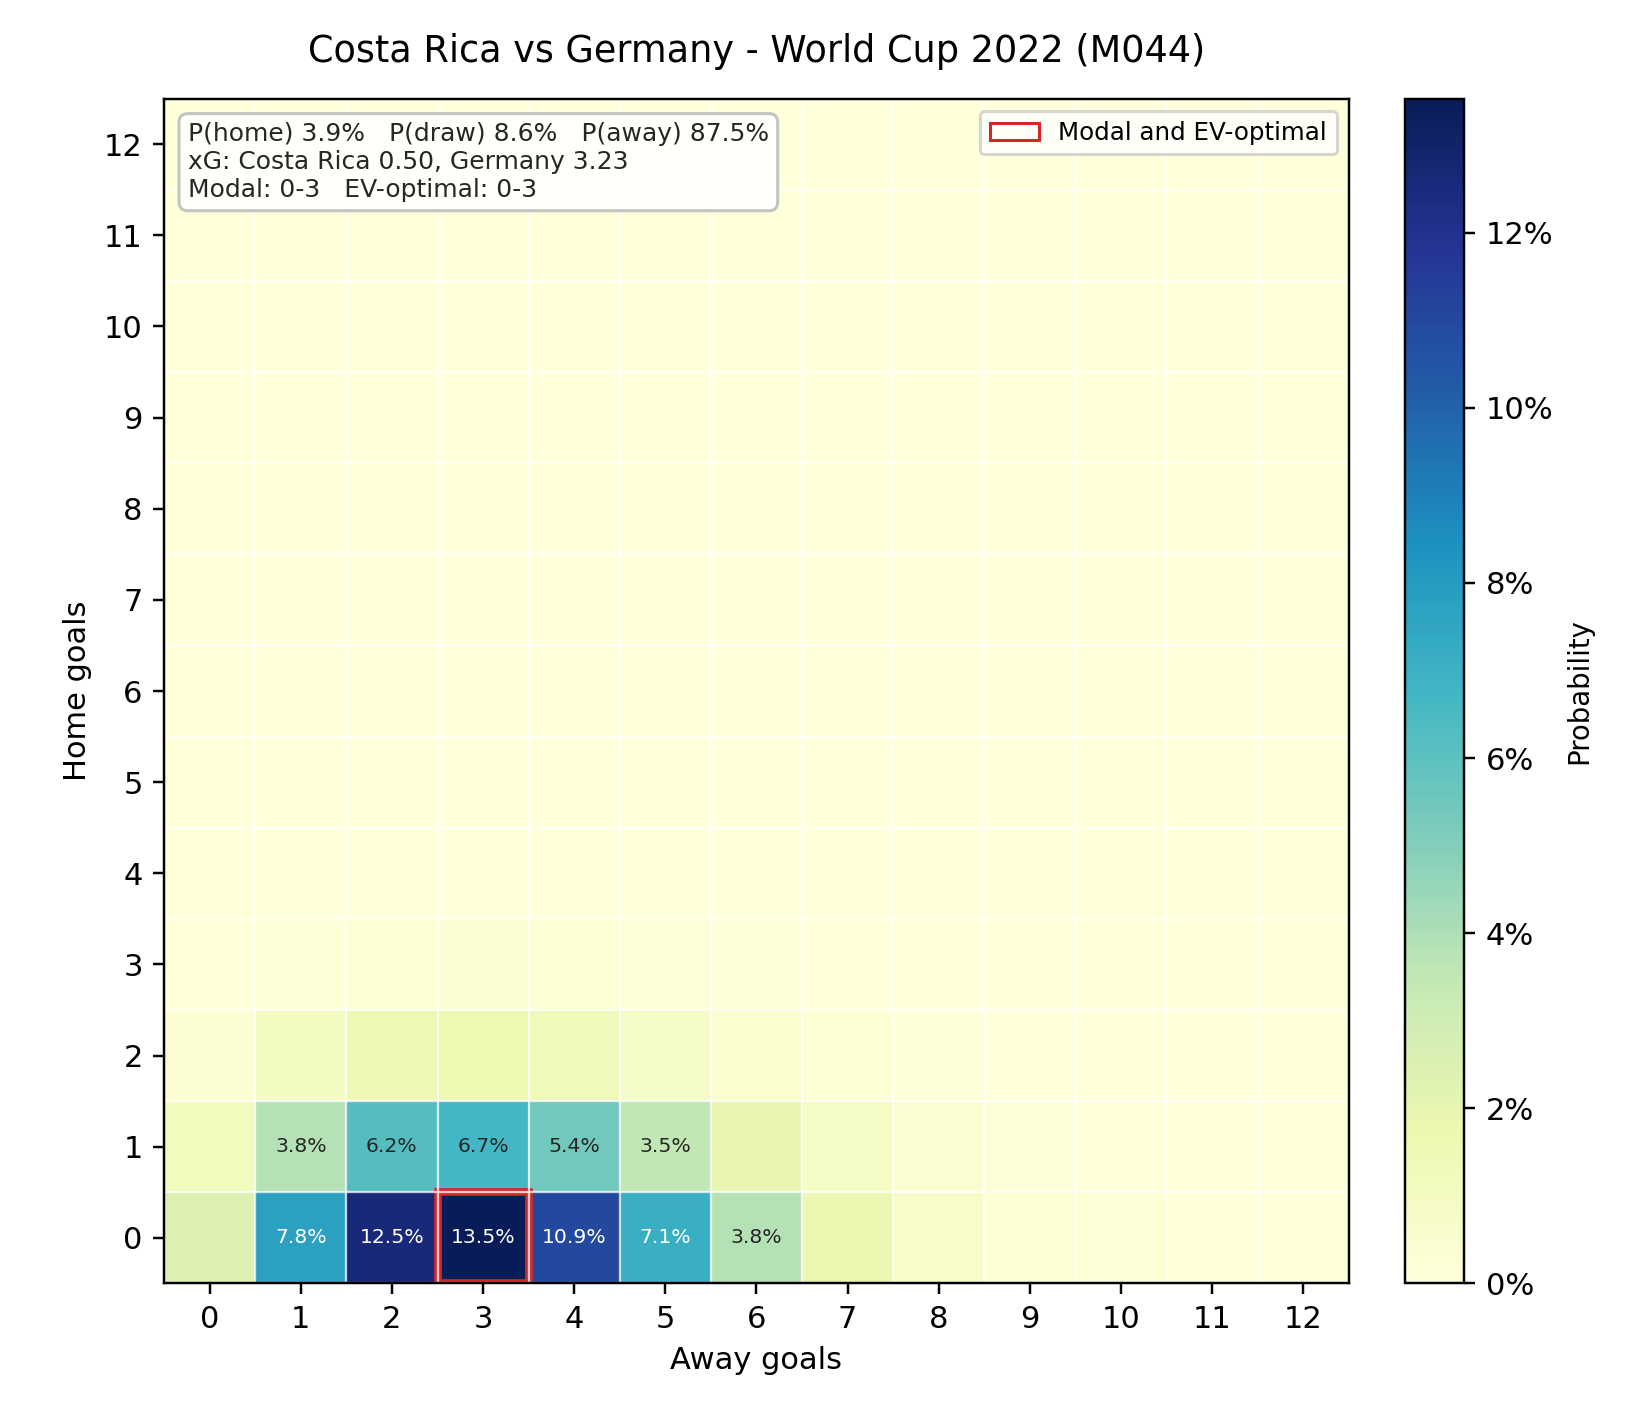
\includegraphics[width=\textwidth]{probability_matrix_extreme_favourite.png}
\end{minipage}\hfill
\begin{minipage}{0.5\textwidth}
\centering
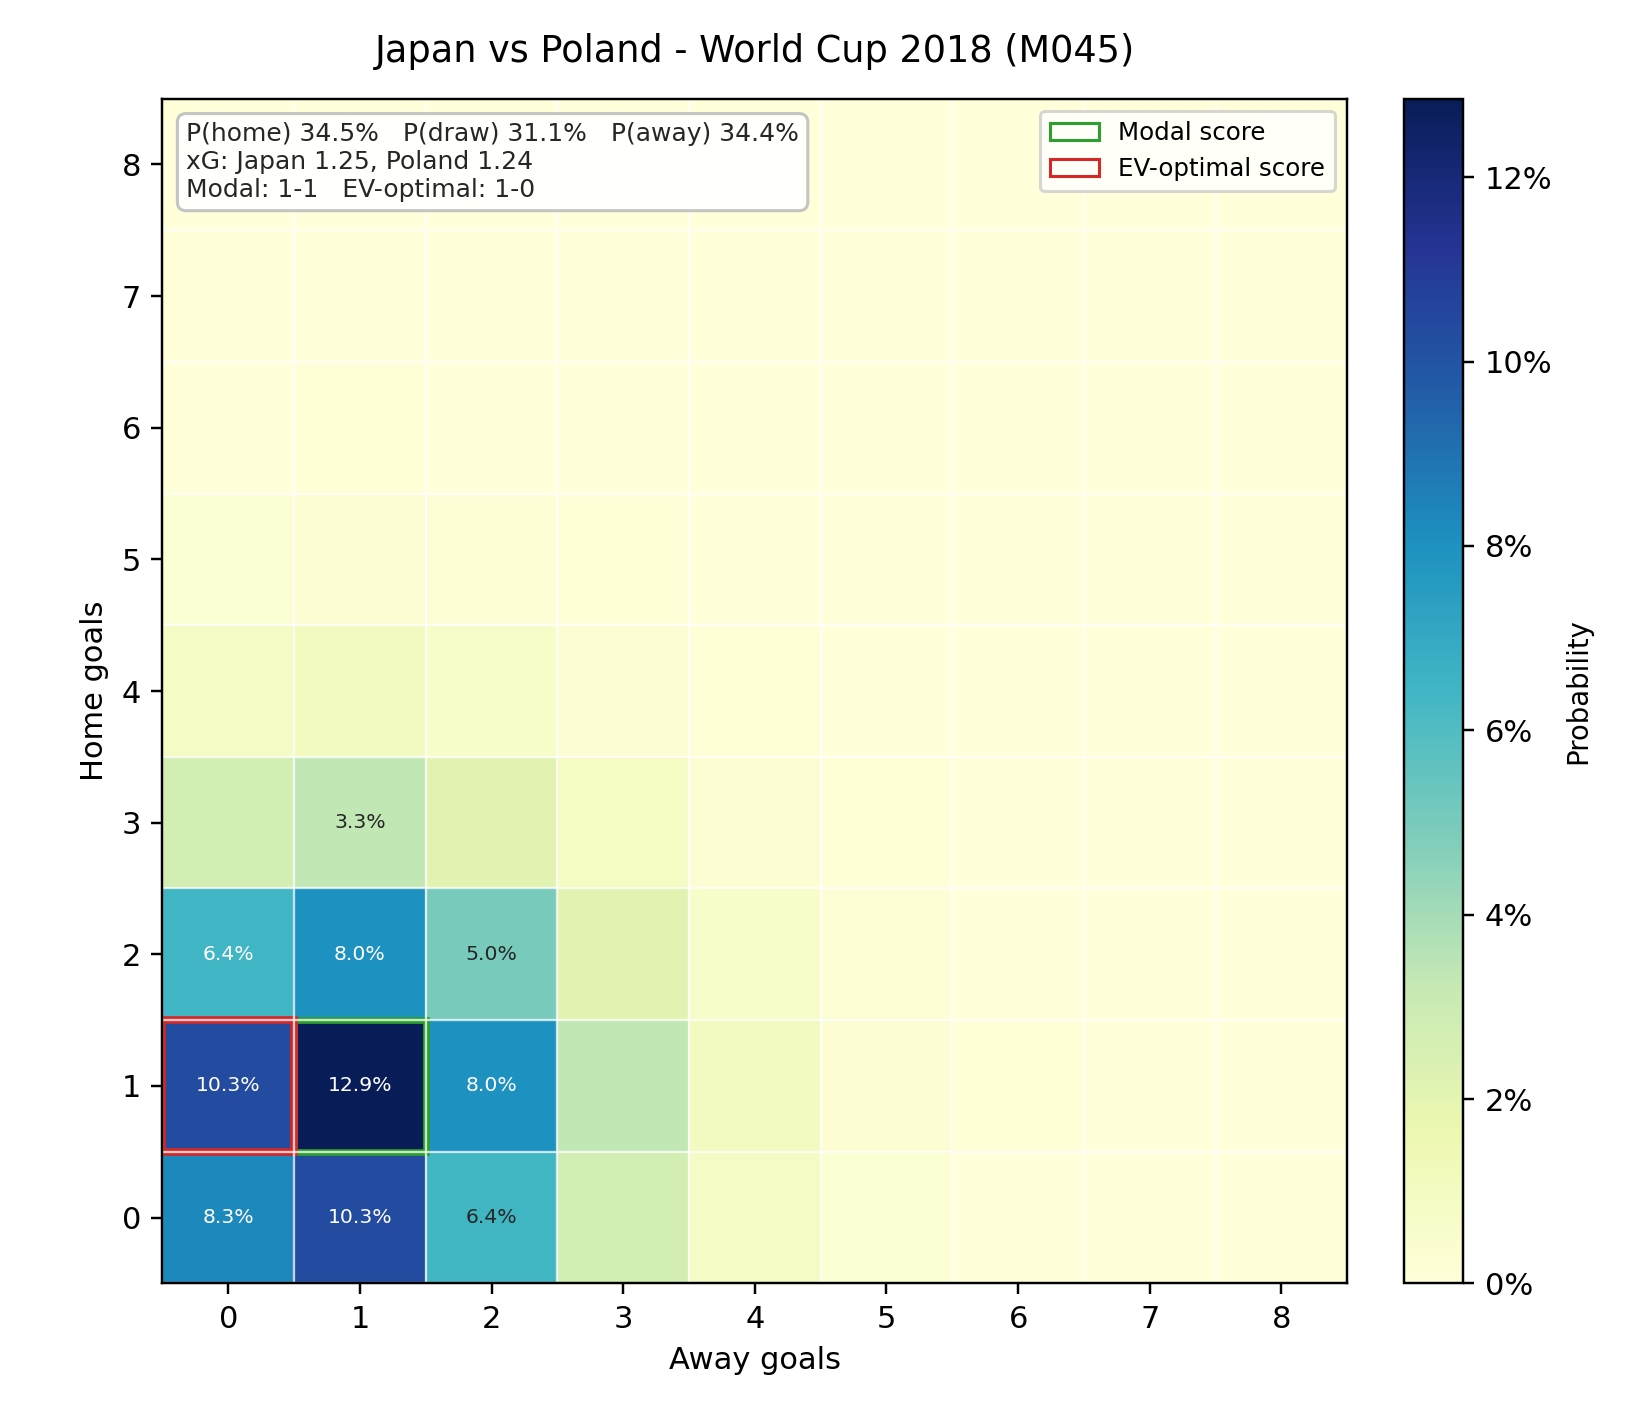
\includegraphics[width=\textwidth]{probability_matrix_balanced.png}
\end{minipage}
\caption{Representative exact-score probability matrices from the baseline Poisson pipeline. The left panel shows the highest favourite-probability match in the historical sample, while the right panel shows the most balanced team A/team B win-probability match. The red outline marks the expected-points-optimal score; when distinct, the green outline marks the modal scoreline. The balanced example uses the default \(G=8\) grid, while the extreme-favourite example is displayed on the larger diagnostic grid to show high-margin tail mass.}
\label{fig:probability-matrices}
\end{figure}

\section{Market calibration targets}
\label{sec:calibration}

Calibration chooses $(\lambda_X,\lambda_Y)$ so that quantities implied by the matrix match
the corresponding market-implied probabilities. The relevant matrix functionals are
\begin{align}
\Prob(X>Y)&=\sum_{x>y}\pi_{xy}, &
\Prob(X=Y)&=\sum_{x=y}\pi_{xy}, &
\Prob(X<Y)&=\sum_{x<y}\pi_{xy}, \label{eq:1x2}\\[2pt]
\Prob(X>0,Y>0)&=\sum_{x>0,y>0}\pi_{xy}, &
\Prob(X+Y>L)&=\sum_{x+y>L}\pi_{xy}, \label{eq:bttsou}
\end{align}
for the result (1X2), BTTS, and total-goals lines respectively; the goal margin $X-Y$ and
selected correct-score cells $\pi_{xy}$ supply further targets. The calibration minimises a
weighted squared error between these model quantities and their market-implied counterparts,
\begin{equation}
(\lambda_X,\lambda_Y)
=\arg\min_{\lambda_X,\lambda_Y}\;
\sum_{k}\omega_k\big(f_k(\lambda_X,\lambda_Y)-m_k\big)^2,
\label{eq:calibration}
\end{equation}
where $f_k$ is a model functional from~\eqref{eq:1x2}--\eqref{eq:bttsou}, $m_k$ is the
market target, and $\omega_k$ is a reliability weight that prioritises the most liquid
markets (result first, then totals and BTTS).

\paragraph{Why 1X2 alone does not identify total-goal intensity.} The 1X2 market fixes only
three aggregate result probabilities: team A win, draw, and team B win. Many different
scoreline matrices can share the same three result probabilities while having different
expected total goals, BTTS probabilities, and high-score tail mass. Even within an independent
Poisson family, the result probabilities mostly constrain relative team strength and the
draw mass; total-goal intensity is then inferred indirectly rather than observed from a
direct totals price. A 1X2-only calibration is therefore useful as a common-information
baseline, but it does not fully identify the level or shape of the score distribution.

The fit is deliberately \emph{overidentified}: the two intensities
$(\lambda_X,\lambda_Y)$ are calibrated against many more market constraints than there are
parameters (result, several total-goals lines, BTTS, and indirectly margin and
correct-score information). A two-parameter independent-Poisson model therefore
\emph{cannot} reproduce all of these markets exactly and simultaneously; the weighted
objective in~\eqref{eq:calibration} returns the best compromise, with $\omega_k$ deciding
which markets are matched most closely when they disagree. Any residual discrepancy between
a model functional and its market target is expected and is reported as a calibration
diagnostic rather than forced to zero. This is the same logic by which a parsimonious
financial model is calibrated to liquid instruments: the market is the data, and the
low-parameter model is a smooth, internally consistent interpolation of it that need not,
and generally will not, fit every quoted instrument perfectly. Closer agreement with several
markets at once is one role of the market-consistent projection of
Section~\ref{sec:entropy}, which relaxes the strict two-parameter form.

Richer markets such as totals, BTTS, correct score, and Asian handicap therefore constrain
dimensions of the scoreline distribution that 1X2 probabilities do not pin down.

\section{Correct-score market information}

Correct-score markets price individual cells of $\pi$ directly and therefore look like the
most informative source of all. In practice they are noisy inputs: they often carry large overrounds, quote only a sparse subset of scorelines, and may be affected by demand for salient or popular scores. 
We therefore treat correct-score odds as useful but noisy evidence rather than ground truth. In the simplest representation the market and model matrices are blended
schematically as
\begin{equation}
\pi^{\mathrm{blend}}_{xy}=w\,\pi^{\mathrm{model}}_{xy}+(1-w)\,\pi^{\mathrm{CS}}_{xy},
\qquad w\in[0,1],
\label{eq:blend}
\end{equation}
where $\pi^{\mathrm{CS}}$ is the devigged, renormalised correct-score matrix over the quoted
cells. Equation~\eqref{eq:blend} is conceptual: the actual treatment handles the quoted cells
and the unquoted tail / ``Other'' mass with more care, but the modelling idea --- shrinking the
model matrix toward direct correct-score evidence by a trust weight $w$ --- is captured by it.
The live policy keeps $w=1$ (model only). In diagnostic sweeps the blend was researched across
several weights; the evidence did not justify changing the default, so correct-score blending
remains a research diagnostic.

\section{Asian handicap and margin information}

Asian handicap markets price the realised goal margin $M=X-Y$ (the same quantity used in the
scoring decomposition) and are structurally aligned with the goal-difference tier. For a
team A handicap $h$, define the handicap-adjusted margin $M_h=M+h$. A unit stake on team A at
decimal odds $O$ then settles as
\begin{equation}
\Pi=
\begin{cases}
O-1, & M_h>0,\\
0,   & M_h=0,\\
-1,  & M_h<0,
\end{cases}
\label{eq:ah}
\end{equation}
with team B taking the opposite side. Quarter lines (for example $h=-3.25$) are handled as
two equal half-stake bets on the adjacent half and integer lines. After two-way margin
removal, the fair handicap odds make the expected settled profit zero under the market's
own implied margin distribution, which yields a constraint on $\pi$ through the margin law
$\Prob(M=k)=\sum_{x-y=k}\pi_{xy}$.

Asian handicap is genuinely relevant because it is the market that most directly prices the
quantity the $7$-point tier rewards. However, our analysis is conservative. Using the actual
quoted main handicap line (rather than an interpolated one), a tendency for favourites to
under-cover the implied margin was weak, not statistically significant, and concentrated in a
small subset of line types; it is treated as a monitor-only observation and is \emph{not}
used as a blanket favourite-fade rule. Asian handicap enters the model only as margin
information for the market-consistent challenger described next.

\section{Market-consistent matrix as an entropy projection}
\label{sec:entropy}

The market-consistent challenger refines a prior scoreline matrix $Q$ (typically the
calibrated Poisson matrix) into a posterior $P$ that stays close to the prior while better
matching a set of market constraints. This is a minimum-relative-entropy / entropy-pooling
problem in the spirit of entropy pooling \cite{meucci2008}, using the Kullback--Leibler divergence
\cite{kullbackleibler1951}
\[
\KL(P\,\|\,Q)=\sum_{x,y}P_{xy}\log\frac{P_{xy}}{Q_{xy}} .
\]
With reliability-weighted soft constraints it takes the form
\begin{equation}
\min_{P}\;
\KL(P\,\|\,Q)
+\sum_{k}\omega_k\big(f_k(P)-m_k\big)^2
\qquad\text{s.t.}\qquad
P_{xy}\ge 0,\;\sum_{x,y}P_{xy}=1,
\label{eq:entropy}
\end{equation}
where the $f_k(P)$ are model-implied market quantities (result, totals, BTTS, selected
correct-score cells, and Asian-handicap expected-profit conditions), the $m_k$ are their
market targets, and the $\omega_k$ encode how much each market is trusted. The KL term keeps
the adjustment minimal --- $P$ departs from the transparent Poisson prior only as far as the
market evidence warrants --- while the penalty terms pull the implied quantities toward the
market.

It is worth recording the exact-constraint limit, which has an elegant closed form. If the
penalties are replaced by hard linear moment constraints $\sum_{x,y}P_{xy}f_k(x,y)=m_k$, the
minimum-relative-entropy projection of $Q$ onto those constraints is an exponential tilt of
the prior,
\begin{equation}
P_{xy}=\frac{Q_{xy}\,\exp\!\big(\sum_k \theta_k\, f_k(x,y)\big)}{Z(\theta)},
\qquad
Z(\theta)=\sum_{x,y}Q_{xy}\,\exp\!\Big(\sum_k \theta_k\, f_k(x,y)\Big),
\label{eq:gibbs}
\end{equation}
where the $\theta_k$ are Lagrange multipliers fixed by the constraints and $Z(\theta)$
normalises the distribution. The problem is convex in $P$, and~\eqref{eq:gibbs} is recovered
by solving its finite-dimensional convex dual in $\theta$; this is the Gibbs / exponential-family
form familiar from maximum-entropy inference and entropy pooling. The implemented
soft-constraint version~\eqref{eq:entropy} is a reliability-weighted, regularised analogue of
this projection: finite weights $\omega_k$ play the role of soft multipliers, trading exact
moment matching for robustness to noisy or mutually inconsistent market targets. 

Prior challenger diagnostics found the market-consistent matrix \emph{including}
Asian-handicap constraints worth monitoring, but any gains were small and depended on the
optimiser reaching an acceptable fit. It is therefore used as a \emph{gated} challenger,
surfaced only when its fit status is acceptable, and never as the silent default.

\section{Challenger models and diagnostics}
\label{sec:challengers}

Around the EV-optimal default sits a set of challenger views and flags, all of which inform a
human decision without automatically overriding $p^{*}$:
\begin{itemize}
\item \textbf{Modal / most-likely scoreline:} $\arg\max_{x,y}\pi_{xy}$, the single most
probable score; a manual-review alternative, not a default.
\item \textbf{Dixon--Coles low-score adjustment:} a multiplicative correction to the
$\{0\text{-}0,1\text{-}0,0\text{-}1,1\text{-}1\}$ cells capturing dependence in low-scoring
games \cite{dixoncoles1997}, with the dependence parameter estimated from low-score market
cells where available.
\item \textbf{Larger-grid diagnostic:} a recomputation on a wider goal grid to quantify
truncated tail mass for extreme favourites.
\item \textbf{Draw-prone flag:} a balanced result probability combined with a low expected
total, marking matches where the EV pick is a fragile decisive score.
\item \textbf{Blowout-risk flag:} a strong favourite with a high expected total, used to
surface higher-margin alternatives.
\item \textbf{BTTS-conflict flag (narrowed):} a no-BTTS EV pick alongside an elevated BTTS
probability and a close BTTS-compatible alternative; a difficulty note only.
\item \textbf{Round-3 favourite-fade note:} a review note motivated by group-stage
qualification incentives, not an automatic adjustment.
\end{itemize}
The governance is intentional. With a small historical validation sample, a diagnostic that
looks helpful can easily be a small-sample artefact, so challengers are kept as explainable
signals rather than promoted to overrides without robust, cross-tournament evidence.

\section{Historical validation}
\label{sec:validation}

Consistently available historical inputs differ by tournament. The validation therefore
separates two layers: an extended 2014/2018/2022 Football-Data layer restricted to average
1X2 odds, and a richer 2018/2022 diagnostic layer using auxiliary-market inputs. The former
expands the sample for the core decision-layer comparison; the latter supports the governance
status of auxiliary-market challengers.

The extended layer uses the available Football-Data World Cup workbook as the source for
the 2014, 2018, and 2022 validation extension.\footnote{Historical odds and results from
Football-Data, \url{https://www.football-data.co.uk}.} The workbook contains sheets for the
2014, 2018, and 2022 World Cups, but no 2010 sheet. The reported extension therefore covers
\[
144\ \text{group-stage matches}\ (48+48+48),
\]
not 192. This is a deliberately common-input validation: only the 1X2 market is used, with
Football-Data's average odds columns \(H\)-Avg, \(D\)-Avg, and \(A\)-Avg available for every
loaded row. Each loaded match carried complete average 1X2 odds. Realised scores are taken
from the full-time score columns HGFT and AGFT only.

This Football-Data extension reconstructs an independent-Poisson score matrix from the
average 1X2 probabilities, scores each prediction under~\eqref{eq:scoring}, and compares the
modal scoreline with the expected-points scoreline. Asian-handicap, correct-score, and
market-consistent-with-Asian-handicap (MC+AH) logic is not applied in this extension because
comparable inputs are not present for these tournaments. Table~\ref{tab:results} summarises
the realised pool points and should be read as descriptive validation evidence rather than as
a statistically decisive ranking.

\begin{table}[htbp]
\centering
\small
\begin{tabular}{lrrrr}
\toprule
Strategy & 2014 & 2018 & 2022 & Combined \\
\midrule
Most likely / modal          & 190 & 227 & 190 & 607 \\
EV-optimal 1X2               & 193 & 222 & 179 & 594 \\
EV-optimal 1X2 + O/U slot    & 193 & 222 & 179 & 594 \\
\bottomrule
\end{tabular}
\caption{Realised group-stage pool points in the Football-Data 1X2-only validation across
the 2014, 2018, and 2022 World Cups (\(n=144\)). The modal scoreline has the highest realised
total over this specific sample, but realised points are high variance and do not by
themselves overturn the ex-ante expected-points decision rule. The O/U-slot variant matches
the plain EV-optimal row because the Football-Data extension provides no totals market for
the slot to act on.}
\label{tab:results}
\end{table}

The modal scoreline outscored the EV-style predictions over this particular 144-match sample,
with a combined realised total of 607 points versus 594. This is an empirical outcome of the
sample, not a change in the decision rule. Equations~\eqref{eq:decisive}--\eqref{eq:draw}
define the ex-ante expected-points objective under the pool payoff; the EV-optimal prediction
remains the rule that maximises expected points conditional on the estimated scoreline
distribution. The modal prediction remains useful as a manual-review challenger, especially
in balanced or draw-prone matches, but the realised 144-match ranking is not strong enough to
promote it to the live default. The existing governance of richer challengers is unchanged:
MC+AH remains a gated challenger when its inputs and optimiser fit are acceptable,
correct-score blending remains research-only, and no betting-alpha claim is made.

Table~\ref{tab:richer-diagnostics} records the richer 2018/2022 diagnostic layer separately.
These rows use auxiliary-market inputs and research configurations that are not available in
the Football-Data extension, so they should not be read as part of the \(n=144\) headline
comparison. They re-ground the challenger policy: small realised gains from MC+AH and
correct-score blending are monitored, power devig is not promoted, and Dixon--Coles /
larger-grid diagnostics remain inert on the tested combined sample.

\begin{table}[htbp]
\centering
\small
\begin{tabular}{lrp{0.48\textwidth}}
\toprule
Strategy / diagnostic & Points & Governance interpretation \\
\midrule
EV-optimal default        & 391 & Live default benchmark \\
Modal / most-likely       & 412 & Manual-review challenger; realised gain does not overturn EV policy \\
Market-consistent $+$ AH  & 399 & Gated challenger; small fit-dependent gain \\
Correct-score blend       & 400 & Research-only; not promoted to default \\
Power devig               & 386 & Underperforms; not recommended for serious live use \\
Dixon--Coles / larger grid & 391 & Inert relative to default on this combined diagnostic layer \\
\bottomrule
\end{tabular}
\caption{Richer 2018/2022 diagnostic layer, not the headline Football-Data extension. These
realised pool-point totals use auxiliary-market research outputs from the 2018 and 2022
group stages (\(n=96\)) and inform challenger governance only; they do not establish a
betting edge or override the ex-ante expected-points default.}
\label{tab:richer-diagnostics}
\end{table}

\subsection*{Probabilistic validation as a complementary layer}

Realised pool points measure the right thing --- the quality of the \emph{contest decision} ---
but they are a high-variance estimator. A single match contributes a discrete payoff in
$\{1,5,7,10\}$, an exact hit is rare, and a tournament's worth of draws or upsets can move a
strategy's total by more than any plausible model edge. Ranking strategies on points alone at
\(n=144\) still risks rewarding luck. We treat realised points as the headline contest metric
and recommend, as a complementary layer, evaluating the quality of the implied distribution
$\pi$ with \emph{proper scoring rules} and calibration analysis, which are far less sensitive to
the discrete payoff:
\begin{itemize}
\item the \emph{Brier score} and \emph{log loss} on the result probabilities
$\big(\Prob(X>Y),\Prob(X=Y),\Prob(X<Y)\big)$, rewarding sharp and well-calibrated forecasts;
\item the \emph{Ranked Probability Score} (RPS), the standard metric for ordered football
outcomes, which penalises probability mass placed far from the realised result and so respects
the natural ordering loss--draw--win;
\item \emph{reliability (calibration) curves} of realised frequency against implied probability
by bucket, together with the calibration--refinement decomposition of the Brier score, which
separates ``are the stated probabilities honest?'' from ``are they informative?''.
\end{itemize}
The two layers answer different questions and should be read together: realised points evaluate
the decision taken under the scoring rule, while proper scores and calibration evaluate the
distribution from which that decision was derived. A variant can improve calibration without
improving realised points, or win points through variance while being no better calibrated; only
the combination distinguishes signal from luck.

\paragraph{Reported probability quality.} This layer is implemented for the same Football-Data
1X2-only validation. Table~\ref{tab:prob} summarises the proper-score results by tournament
and combined sample. The combined 1X2 Brier score is \(0.570\), log loss \(0.971\), and RPS
\(0.138\). The 2022 tournament is the least favourable of the three by these metrics, with
Brier \(0.601\), log loss \(1.032\), and RPS \(0.149\). At this sample size the figures are
best read as a sanity check that the average 1X2 market probabilities are plausible inputs,
not as evidence of a market-beating probability model.

\begin{table}[htbp]
\centering
\small
\begin{tabular}{lcccc}
\toprule
Sample & Matches & Brier & Log loss & RPS \\
\midrule
2014     & 48  & 0.563 & 0.951 & 0.135 \\
2018     & 48  & 0.547 & 0.931 & 0.131 \\
2022     & 48  & 0.601 & 1.032 & 0.149 \\
Combined & 144 & 0.570 & 0.971 & 0.138 \\
\bottomrule
\end{tabular}
\caption{Probabilistic validation for the Football-Data 1X2-only extension on the 2014, 2018,
and 2022 group stages and their combined sample (\(n=144\)). The reported quantities are 1X2
proper scores only: Brier score, clipped log loss, and Ranked Probability Score (RPS).}
\label{tab:prob}
\end{table}

Figures~\ref{fig:calibration} and~\ref{fig:goals} give complementary visual checks on the
validation layers. The reliability plot buckets the Football-Data average-odds 1X2
probabilities into favourite, draw, and underdog classes. The goals plot compares realised
mean total goals with the mean total implied by the renormalised score matrix, computed as
\(\sum_{a,b}\pi_{ab}(a+b)\). The Football-Data extension is intentionally restricted to
average 1X2 odds, which are available consistently across the 2014, 2018, and 2022
tournaments. This restriction is useful for sample-size expansion, but it also reduces the
information available for scoreline calibration: total-goal intensity must be inferred
indirectly from win/draw/loss probabilities.

The 1X2-only matrix is somewhat conservative on total goals in this sample. The combined
expected mean is \(2.387\) goals per match versus \(2.625\) realised, a realised-minus-model
gap of \(0.238\) goals, or about \(10.0\%\) relative to the model expectation. The gap is
positive in all three tournaments, largest in 2014 and smaller in 2022, but the sample is too
small to read the tournament-by-tournament pattern as a trend. A simple draw diagnostic points
in the same direction: the average implied draw probability is \(0.245\), while the realised
draw frequency is \(0.194\). This is interpreted as a limitation of inferring a full scoreline
distribution from 1X2 odds alone, rather than as a failure of the expected-points decision
rule. Figure~\ref{fig:goals} therefore also includes an apples-to-apples 2018/2022 comparison
against the richer live-paste validation layer, which includes explicit total-goals market
inputs. On that common 96-match subset, the Football-Data 1X2-only layer has expected mean
total goals of \(2.346\) versus \(2.521\) realised, while the richer layer has \(2.567\)
expected versus \(2.521\) realised. This supports treating the Football-Data extension as a
decision-layer robustness check rather than as a full replacement for the richer
market-input calibration.

\begin{figure}[htbp]
\centering
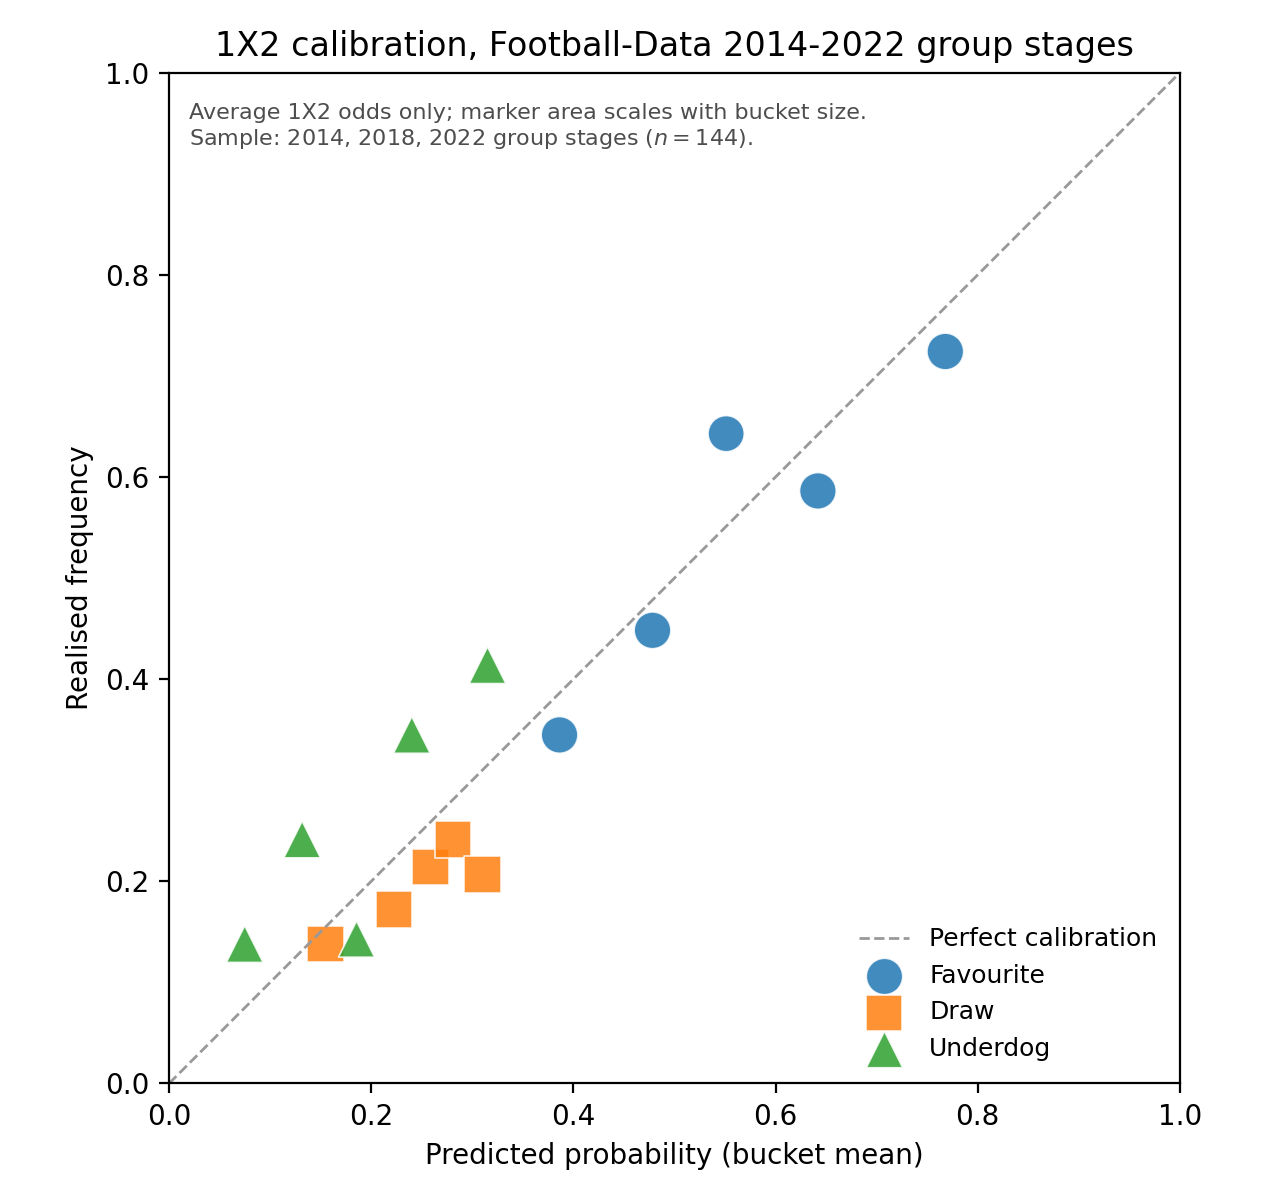
\includegraphics[width=0.62\textwidth]{calibration_1x2.png}
\caption{Reliability of the 1X2 probabilities in the Football-Data average-odds extension
over the 2014, 2018, and 2022 group stages (\(n=144\)). Predicted probability bucket means
are plotted against realised frequencies for favourite, draw, and underdog outcomes, with
marker area scaled by bucket sample size.}
\label{fig:calibration}
\end{figure}

\begin{figure}[htbp]
\centering
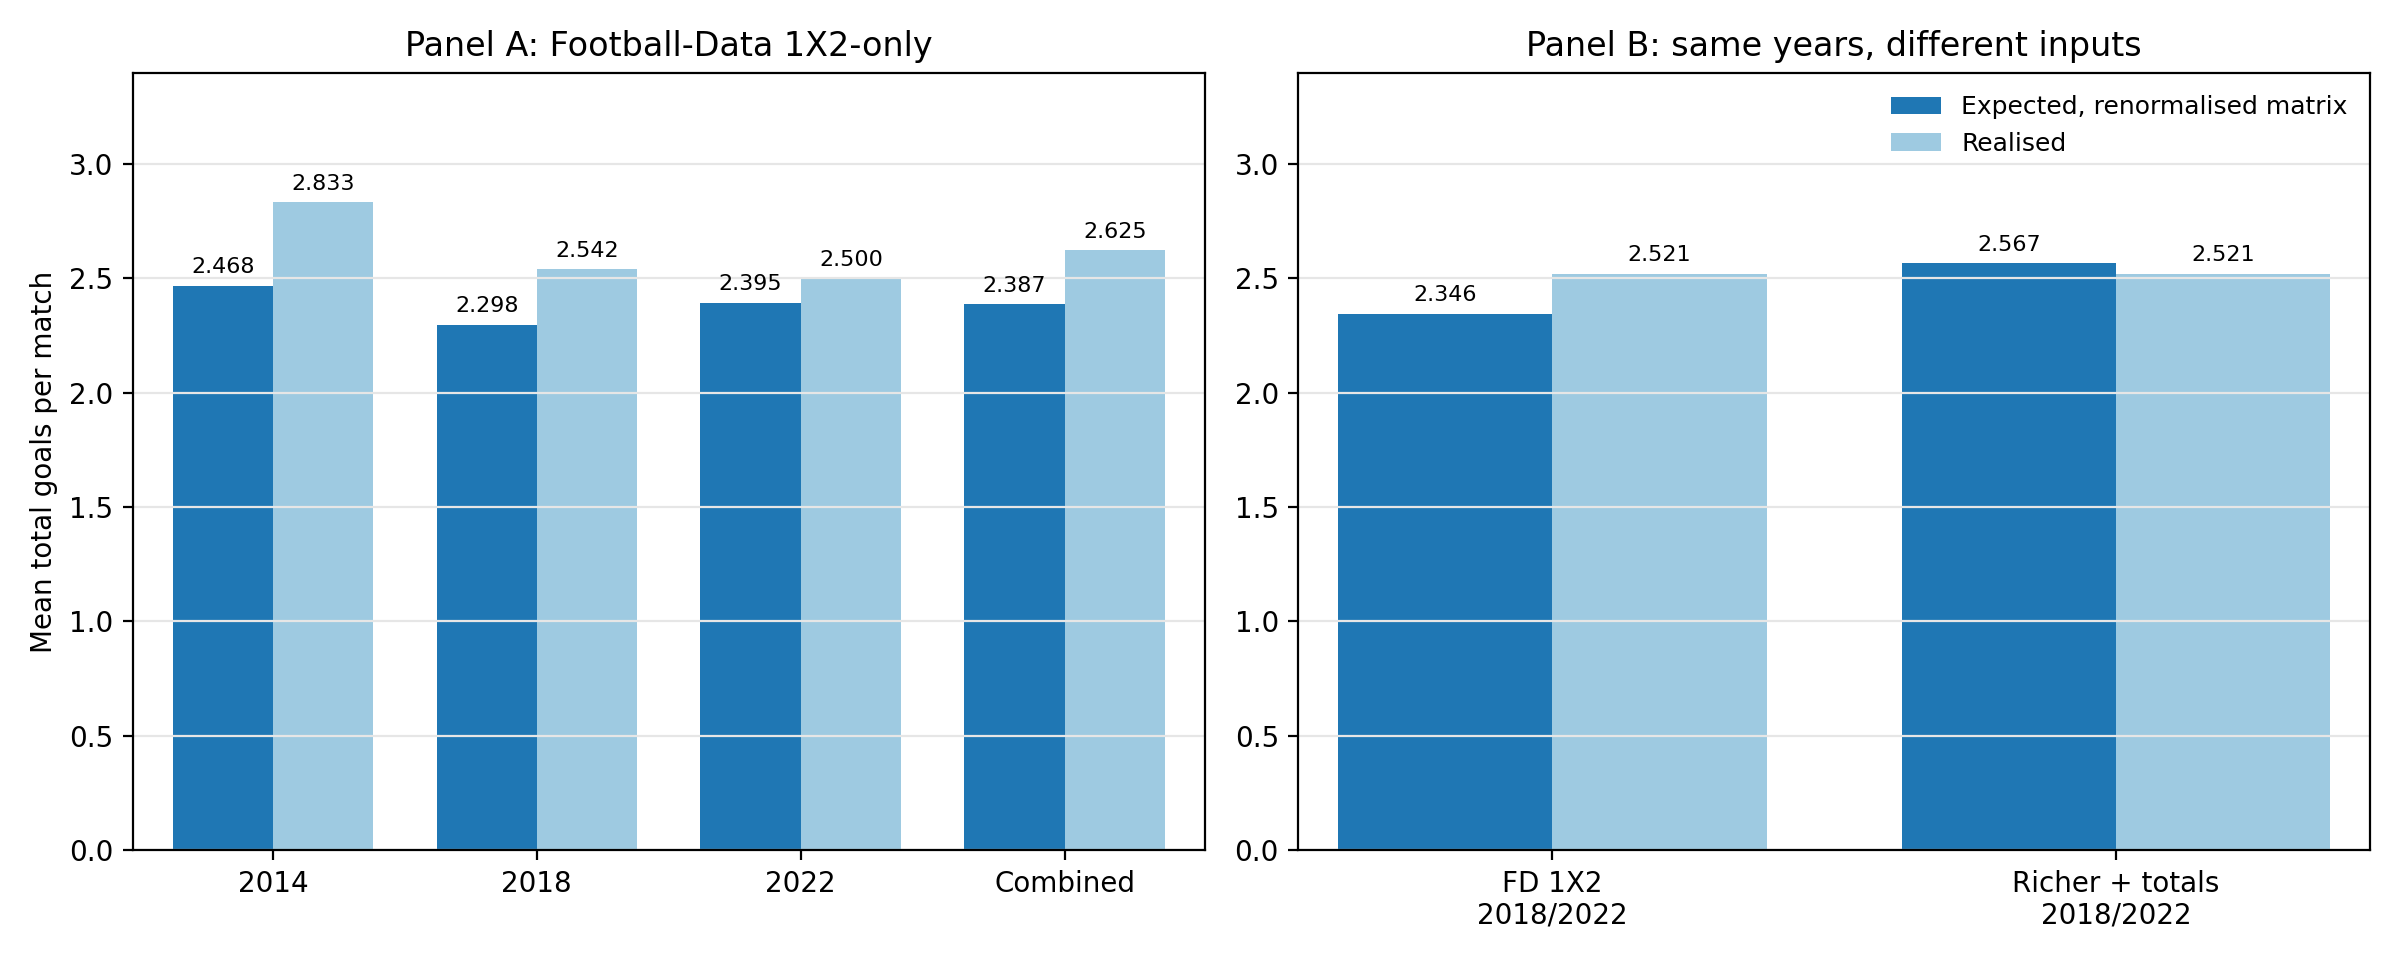
\includegraphics[width=\textwidth]{expected_vs_actual_goals.png}
\caption{Expected versus realised mean total goals. Panel A reports the Football-Data
extension, which uses only average 1X2 odds and therefore infers total-goal intensity
indirectly from win/draw/loss probabilities. Panel B compares the 2018/2022 subset across
validation layers. The richer validation layer, which includes explicit total-goals market
inputs, is much closer to realised mean total goals. The difference illustrates the
information loss in the 1X2-only extension and is not interpreted as a failure of the
expected-points decision rule.}
\label{fig:goals}
\end{figure}

The two panels should therefore be read together: Panel A diagnoses what is lost when the
validation is expanded using only consistently available 1X2 odds, while Panel B shows that
the richer market-input layer largely removes that total-goals bias on the years where both
layers are available.

\paragraph{Distribution quality versus decision governance.} The probabilistic layer makes a
structural point that realised points alone obscure. The probability vectors are almost invariant
across the modal and EV-style strategies in the Football-Data extension: they are different
scoreline-selection rules applied to the same 1X2-calibrated distribution. Their realised-points
differences therefore arise from \emph{decision governance under the payoff function}, not from
different probability estimates. The probabilistic table does not evaluate Asian-handicap,
correct-score, BTTS, or total-goals information, because those inputs are not used in this
extension.

\paragraph{Scope caveat.} The 144-match extension is intentionally narrower than the live
prediction pipeline. It validates the common 1X2 baseline using average Football-Data odds and
HGFT/AGFT realised scores. Correct-score blend weights, MC+AH, Asian-handicap margin signals,
BTTS conflict flags, and total-goals diagnostics are not exercised in these results and are not
claimed as validated by Table~\ref{tab:results} or Table~\ref{tab:prob}.

\subsection*{Statistical uncertainty}

The combined sample of \(n=144\) group-stage matches is useful but small, and the realised-points
gaps in Table~\ref{tab:results} are well within sampling noise: the standard error of a
strategy's mean points per match is of order $0.3$, so totals separated by ten or twenty points
over this sample are not distinguishable with confidence. The appropriate inference tool for
such strategy gaps is a paired bootstrap over matches, which yields confidence intervals on the
difference in realised points rather than a point estimate. Small apparent edges that do not
survive such intervals --- or that appear in only one tournament --- should not be promoted to
the live default. This is precisely the reasoning behind the conservative governance policy
below: the burden of proof for changing the default is cross-tournament, out-of-sample evidence,
not in-sample ranking.

\section{Discussion}

The exercise is subtle for reasons that generalise beyond football. First, the optimal action
depends on the payoff, not only on the probabilities: the same matrix $\pi$ yields different
optimal predictions under different scoring rules, and a perfectly calibrated model can still
produce ``unintuitive'' picks. Second, the prevalence of $1\text{-}0$ and $0\text{-}1$
predictions in the EV-optimal output is a property of the scoring rule
(equation~\eqref{eq:decisive}), not evidence that the model underestimates goals; the result
and margin tiers simply reward narrow decisive scores. Third, a variant that wins in one
tournament can lose in another, so cross-sample robustness, not in-sample ranking, is the
correct test. Finally, because tournament match markets are close to efficient, the realistic
source of advantage in a pool is disciplined decision governance --- choosing the action that
is optimal under the rule, and resisting the temptation to over-fit challenger models to a
short history --- rather than aggressive model complexity.

\section{Limitations}

The Football-Data validation covers only the 2014, 2018, and 2022 World Cup group stages; the
combined sample of \(144\) matches is informative but still small, and the available workbook
does not contain a 2010 sheet. This extension is also 1X2-only: it uses average result odds and
does not exercise Asian-handicap, correct-score, BTTS, total-goals, or MC+AH logic. The data
lack qualification-state metadata that would let the round-3 effect be tested properly, and
the odds used are not guaranteed to be synchronised closing prices. Historical odds collection
is manual. The market-consistent optimiser requires fit monitoring; the baseline assumes
conditional independence of the two scores, corrected only mildly by the Dixon--Coles term; and
there is no player-availability or news model. The public-field / leaderboard objective is also
outside the main recommendation: maximising expected points is not the same as maximising the
probability of finishing first in a large public pool, where correlation with the field and
deliberately contrarian choices matter.

A natural second-version extension is to collect synchronised opening and closing odds and
measure \emph{closing-line value} --- whether the model's implied probabilities systematically
improve on the closing price. In market-facing settings, closing-line value is a far
lower-variance test of informational edge than realised match outcomes, because it compares two
prices rather than waiting on a single noisy result. The current project does not collect such
data and makes \emph{no} closing-line-value claim; it is noted only as the most informative
future validation a market-facing version could add. Finally, an exact-score pool is not a
betting market --- the model optimises pool points under a fixed rule --- so none of the above
should be read as a wagering strategy.

\section{Conclusion}

Exact-score prediction can be posed rigorously as expected-points optimisation under a known
scoring rule. Devigged bookmaker odds provide a market-implied probability backbone; a
calibrated, transparent scoreline distribution turns those prices into a coherent matrix; and
the prediction is chosen by maximising expected points rather than by reporting the most likely
score. Historical validation on the 2014, 2018, and 2022 World Cup group stages supports a
conservative, gated policy: the expected-points-optimal prediction is the live default, while
modal, market-consistent, Asian-handicap, and correct-score variants serve as challenger
diagnostics or gated alternatives. The most durable conclusion is methodological --- in a
near-efficient market with a small validation sample, careful decision governance is worth more
than additional model machinery.

\section*{AI assistance statement}

Generative AI tools, including ChatGPT, Claude and Codex, were used as assistants during the development of this project. Their use included mainly code drafting, debugging support, and documentation review. All modelling choices, empirical checks, interpretation of results, and final text are the responsibility of the author.

\bibliographystyle{plain}
\bibliography{references}

\end{document}
